Artificial neural networks (ANN) are inspired by the idea of developing programs that are able to learn how to perform certain tasks by getting examples. Neural networks generally don't have any task-specific rules implemented, they learn the important features by themselves. 

The basic idea is to model the neurons in a biological brain. Such artificial neurons (also called connected units or nodes) are linked to each other and transmit signals. The neuron receives the signal and combines it with a certain weight and bias before sending it to the next connected unit. The weight and the bias are free parameters which have to be optimized by the network during the training phase. 
In ANNs, nodes are combined into layers. The input data is processed by several layers connected to each other. Each layer is typically trained to extract a certain feature of the input data to yield the required information at the end. 

Neural networks are mostly used for two different types of analysis. The first one is the prediction of a continuous variable, which is called a regression problem. The second, which is specified here, is the problem of identifying an input as part of a class, called a classification model.
In classification problems the training is typically supervised. The network is given input data and corresponding label vectors which state to which category the respective input belongs. False labelling is penalized and leads to weight and bias adjustments.

Training a network means giving examples of the task and evaluating the performance of the network. This evaluating is done through backpropagation. The input propagates through the network until it reaches the output layer. There it is compared to the actual output vector. The difference between these two or the classification error is given by a loss function. This error is then propagated backwards through the network until every neuron has an associated error value. Through this value the weight and bias of the corresponding neuron is then changed to improve the performance of the network. 

As updating the weights after every input sample is inefficient and makes the loss function very noisy, several samples are combined in one batch or minibatch. The training values are averaged over the sample and the network learns more general features. 

Typically the available input data is limited and can not be easily generated. The network therefore uses the same data several times during the training. One training session which uses the entire data set exactly once is called an epoch. To fully train a ANN several hundred epochs are needed. To prevent the network only being able to classify the training data correctly a small part of it is being split off. This data set is called the validation data. After every epoch the network evaluates its progress on the validation data which has not been used during training. This secures an independent evaluation.  

In contrast to the free parameters set by the network, hyperparameters have to be specified before training starts. Different kinds of networks have different hyperparameters, one of the most important ones being the topology of the network itself. Optimized hyperparameters contribute significantly to the success of a network \cite{Bishop2016}.


\section{Image recognition}
Image recognition has always played a huge part in the development of neural networks. Current state-of-the-art networks in image recognition have partly reached human or even superhuman performance. Image recognition with neural networks is normally placed within the \enquote{deep learning} category. Such architectures include successive layers with nonlinear processing units. Each layer is connected to its predecessor and uses the output of the latter as input. This enables the network to learn different features, higher layers then correspond to higher levels of abstraction. 

In conventional ANNs the neurons are fully connected, meaning that every node in one layer is connected to every node in the layer before and after. The number of weights per node is equivalent to the product of width, height and colours of the picture. They therefore scale very badly to higher resolution images. Fully connected layers can also not take localized characteristics into account. In image recognition neighbouring pixels are more important for feature detection than those far apart.
The problem with conventional multilayer perceptrons is the computing power needed. Therefore, convolutional neural networks (CNNs) have been introduced into image recognition.
Convolutional neural networks can solve both problems stated before and are currently the best performing networks for image recognition \cite{imagenet}. 



\section{Convolutional neural networks}

\begin{figure}
\centering
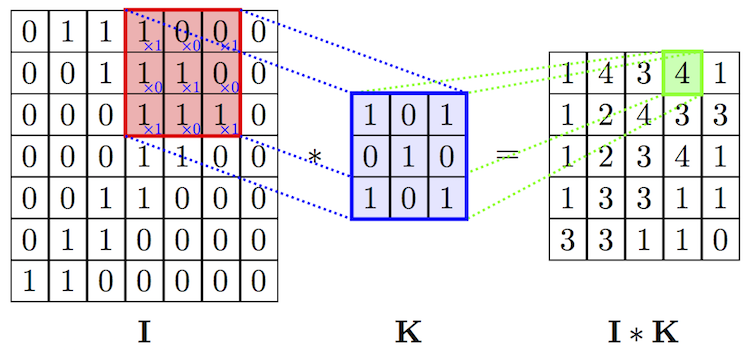
\includegraphics[scale=1.5]{convolve.png}
\caption{A convolutional layer with its kernel. The elements of the kernel are also called a filter. The kernel moves across the whole input data on the left. The right matrix is the product of input and kernel. \cite{convwindow}}
\label{convwindow}
\end{figure}
A convolutional neural network contains several layers in which one input sample is processed in small receptive fields (as seen in fig. \ref{convwindow}). These receptive fields are most often called kernel or filter. One neuron in the layer corresponds to only this part of the input image in width and height but gets the whole depth of the input volume. The dot product between the entries of the kernel and the input is computed and sent to the neuron. The filter values or weights are free parameters of the network that have to be optimized. For different sets of parameters different features can be detected.
The map of neurons is called the activation map. As several input pixels are passed on to one neuron, the size of the input data gets gradually smaller while it is being processed by the network.

Convolutional neural networks are dominated by three different features which make them ideal for image recognition. The first is the 3D volume of neurons, where they are classified in three dimensions, width, height and depth of colour. This ideally represents a picture. The second is the application of spatial locality. One neuron of a following layer is only connected to a small part of neurons in its predecessor. Therefore the network learns to recognize local patterns. With many such layers stacked the patterns learned get increasingly more global, the first one only recognizing lines, while the last one identifies complete features such as \enquote{cat}, \enquote{dog} or \enquote{mouse}.
At last a convolutional neural network takes translational invariance into account. To classify an image correctly, the position of the object in the image is not important. Therefore all neurons in one convolutional layer share the same weights and bias, that means, the same filter is applied while forwarding the signal. Thus one layer always recognizes the same feature, regardless of its position in the image \cite{lecunimage}. 

The hyperparameters for this kind of ANN, which have to be manually tuned, are firstly the size of the convolutional window. If a size of one in width and height is chosen, the window only takes one pixel into account. A bigger size means more information is being observed. The bigger the window the less localized the features detected are. Smaller windows mean more computing power needed, and may not be able to detect larger objects, especially in high resolution pictures. At times it may be advantageous to choose a non-symmetrical kernel size.

The second hyperparameter is the depth of the output volume. It is possible to choose how often a kernel with a new set of weights will be used on the input data or further on in the network. As one kernel with a set of weights is also called a filter, the number of filters can be manually tuned. The more filters are being used, the more free parameters the network has. This can be beneficial as more details can be learned by the network but also disadvantageous as overfitting, which is explained later, is more likely to occur.

If the kernel size is chosen, the stride must be finetuned as well. The stride is the number of pixels the kernel moves in every direction. If the stride is one, then the window only moves one pixel in one direction each time. For a higher stride, the next position of the kernel window overlaps less with the position beforehand. A high overlap of kernel windows occurs for small strides. This can significantly increase the computing time. If the stride is the same as the dimension of the kernel, then the windows do not overlap. This can result in smaller features being lost during the processing.

When the size of the input volume is not a multiple of the kernel size window, then the output dimensions differ from those of the input. Most of the time it is helpful to pad the input volume with zeros at the edges to preserve the spatial size of the input while going through layers. It is also beneficial to minimize edge effects \cite{lecun-89e}.

\section{Overfitting}
Overfitting is a potential problem of deep-learning networks. By choosing layers with a high number of learnable weights and biases, the number of free parameters is very high compared to the actual number of features learnable. Therefore a network is prone to overfit the training data, performing very well during the training but failing while validating on other data (fig. \ref{accuracy}). 

\begin{figure}
\centering
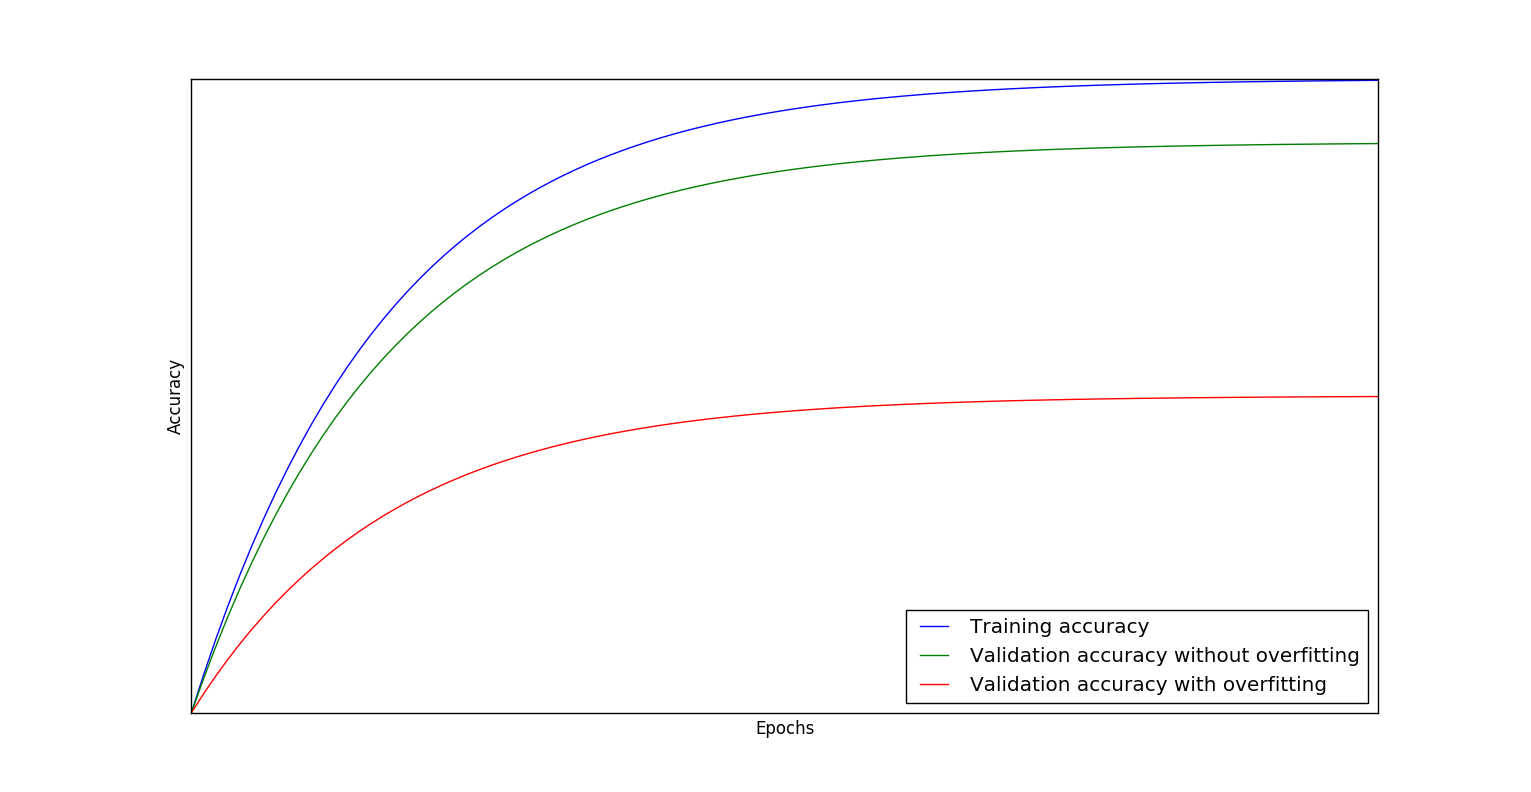
\includegraphics[scale=0.35]{overfittingacc.png}
\caption{Training and validation accuracy. The validation accuracy follows the training accuracy well if there is little or no overfitting. In the case of strong overfitting the validation accuracy increases very little or even decreases during the training.}
\label{accuracy}
\end{figure}
One method to address the problem of overfitting is \enquote{max pooling}. Max pooling also reduces the spatial size, thus limiting the amount of computational power needed. The general idea is that only the rough location in comparison to others of the feature detected is needed, so the input is downsampled with the help of a non-linear function. The working principle is the same as in a convolutional layer. A kernel window moves over the input without overlapping. In every region the activation numbers of the included pixels are compared. The maximum is determined and only this pixel is forwarded to the next layer. For example, in the case of a 2x2 kernel window, the spatial size is reduced by 75 \%, while the depth dimension stays the same. As the network cannot fit parameters to very detailed features, it has to pick up general features, which help correct classification. 

Another method to reduce overfitting is dropout. With dropout a input unit is set to zero before being forwarded to the next layer with a possibility $p$. This is the same as setting the weight of one neuron to zero. This is done after every minibatch of samples, which is tantamount to every parameter update of the network. It forces the network to learn more robust features for a better generalization of the data analysis. Dropout also cuts down on computational time. 

\section{Activation functions}
Deep neural networks need two different kinds of activation functions. The first one is to propagate the signal through the network. After the product between the input signal and the weight of one neuron is computed, the outcome is put into the activation function. Only if a nonlinear activation function is used, non trivial problems can be solved with few nodes. The activation function is applied after every layer, meaning that every output signal is put into relation with the help of the function. The current best working activation function is the ReLu function. ReLu stands for rectified linear unit. It is calculated by
\begin{equation}
f(x) = \mathrm{max} (0,x)
\end{equation}
with x as the input signal. Negative signals are therefore always set to zero while propagating through the network. Other activation functions are for example the sigmoid function or the tangens hyperbolicus. Unlike the ReLu function, those functions saturate when dealing with very high input signals and therefore often perform worse.

The second activation function is needed at the output layer, the last layer in the network. Most deep neural networks are multi-class networks. Multi-class means that the output is not simply signal or background but identifies the input as belonging to one class of several. That means that the output activation function calculates the probability of belonging in each class in correlation to every other probability. A usual activation function in this case is the softmax function. The softmax function calculates a n-dimensional vector of random real values to a n-dimensional vector, where every number lies between 0 and 1 and the sum of all entries is 1. It is calculated by
\begin{equation}
\sigma (\vec{z})_{j} = \frac{\mathrm{e}^{z_j}}{\sum_{k=1}^{n} \mathrm{e}^{z_k} } \quad .
\end{equation}
The vector $\vec{z}$ is the output vector of the neural network, which corresponds after the application of the activation function to $\sigma (\vec{z})_{j}$, the probability of the input belonging to the corresponding classes.
The softmax function cannot be applied if the network is not only multi-class, but also multi-label. The categories in a multi-label network are not mutually exlusive. One input can therefore be classified into several different categories, their probability to fit is not correlated to each other. In this case the beforementioned sigmoid activation function can be used. This function also squashes a vector of real numbers to a vector of real numbers between 0 and 1. In this case the sum of all numbers does not have to be 1. The output $\sigma (\vec{z})_{j}$ is the independent probability of the input data belonging to class j without taking the other classes into account. The function looks like
\begin{equation}
\sigma (\vec{z})_{j} = \frac{1}{1 + \mathrm{e}^{z_j}}  
\end{equation}
with $\mathrm{e}^{z_j}$ as the output vector of the network.
Assigning a class to the input data is normally done by selecting those entries, which have a number higher than 0.5, meaning a probability higher than 50\% of belonging to that class. 
\section{Loss functions}
Loss functions are a way to track the progress while training a neural network. A loss function assigns a real number to the difference between true and estimated class labels of the input, which should be minimized. During training the weights of the neurons are changed according to the increase or decrease of the loss function. For a specific problem it is important to use a suitable loss function. For classification problems such as image recognition with more than two classes, either categorical or binary crossentropy can be used. In machine learning cross entropy is the same as logistic loss. It is calculated by
\begin{equation}
f(x) = y_{\mathrm{true}} \cdot \mathrm{ln} (y_{\mathrm{pred}}) + (1 - y_{\mathrm{true}}) \cdot \mathrm{ln} (1 - y_{\mathrm{pred}})
\end{equation}
where $y_{\mathrm{true}}$ is the true label vector of the input and $y_{\mathrm{pred}}$ the label vector of the prediction of the network.

The difference between categorical and binary crossentropy is only the way in which it is applied. With categorical crossentropy, the whole vector is compared. If only one entry differs, it is considered falsely labeled. This is useful in multi-class problems, where the labels are mutually exclusive. With multi-label problems, binary crossentropy works better. Binary crossentropy compares every label separately, therefore not penalizing one incorrect label so much. 

\section{Optimization algorithms}
To minimize the loss function the neural network has to update its weights and biases during training. This updating is done through an optimization algorithm. To find a minimum of the loss function it is possible to evaluate the gradient of the function. The updating of the network is then proportional to the negative of the gradient. This is an iterative algorithm which finds the steepest descent to a local minimum. The size of the steps taken in the direction of the descent is also called the learning rate. The learning rate is a hyperparameter which has to be optimized to get best training results. 

To compute the gradient for the whole training data takes very long. To shorten the time and computing power needed stochastic gradient descent (SDG) is implemented. SDG uses only one stochastically chosen example to compute the gradient and update the parameters. This can of course result in very varying parameter updates. To prevent this the gradient is computed not over one sample, but over a whole batch. This works because the samples in the dataset are correlated. They all depict the same or similar things, so an update computed for one batch is a good approximation for the complete set. It also can be done much more often, therefore achieving faster convergence for the loss function.

Most optimization algorithms also use momentum. Momentum can be understood by making an analogy to classical physics. If a ball at the top of a hill rolls down, it gains momentum if the direction downhill always stays the same. The hill here represents our loss function. If the gradient of a step points in the same \enquote{direction} as the step before, the \enquote{speed} or step size increases. If the direction changes, the step size gets smaller. If a minimum is found and the imaginary ball oversteps it, the gradient points in the other direction and momentum decreases. The minimum can so be found iteratively.

To further prevent the network from overstepping the minimum which is still a possibility even with momentum, the Nesterov Accelerated Gradient can be implemented. Instead of evaluating the gradient, changing the loss function and then applying momentum, the network anticipates what is going the happen. At first the momentum is applied to the current position. This is an approximation of the future position of the function. At this position the gradient is computed. The network there \enquote{sees} where its going to end up in the next step and can therefore move in the right direction (see fig. \ref{nesterov}). This minimizes the possibility of overstepping and decreases the convergence time. The strength of momentum is also a hyperparameter which needs to be tuned.

\begin{figure}
\centering
\resizebox{!}{5cm}{
\begin{tikzpicture}
%% Linke Hälfte

%Pfeile
\draw [-triangle 60, very thick, red](0,0) -- (5,0);
\draw [-triangle 60, very thick, gruen](0,0) -- (2,4.5);
\draw [-triangle 60, dashed, red, opacity= 0.7] (2,4.5) -- (7,4.5);
\draw[-triangle 60, very thick, blue] (0,0) -- (7,4.5);

%Kugel
\draw[ball color=red] (0,0) node (v1) {} circle (.2);
%\fill[red]  (0,0) ellipse (0.5 and 0.5); Alternative Kugel, mehr ein Kreis

%% Texte
\node[red] at (2.5,-0.5) { \large{gradient step}};
\node[gruen] at (0,3.5) {\large{momentum}};
\node[gruen] at (-0.6,3) {\large{step}};
\node[blue] at (5,2) {\large{actual step}};
\node at (3,6) {\LARGE{Momentum update}};

% Trennlinie
\draw [gray, very thick](9,6.5) -- (9,-1);

%% Rechte Hälfte

%Pfeile
\draw [-triangle 60, gruen, very thick](11,0) node (v2) {} -- (13,4.5) node (v3) {};
\draw [blue, -triangle 60, very thick](11,0) -- (17,3) node (v4) {};
\draw [red, -triangle 60, very thick](13,4.5) -- (17,3);

%Kugel
\draw[ball color=red] (11,0) circle (.2);

%%Texte
\node at (13.5,6) {\LARGE{Nesterov momentum update}};
\node[gruen] at (10.5,3.5) {\large{momentum}};
\node[gruen] at (9.9,3) {\large{step}};
\node[blue] at (15,1) {\large{actual step}};
\node[red] at (15.5,5) {\large{'lookahead'}};
\node[red] at (15.5,4.5) {\large{gradient step}};

\end{tikzpicture}
}
\caption{Classical momentum compared to Nesterov momentum. The network anticipates its future position through momentum and calculates the gradient based on that. It ends up on a slightly different position, thus converging faster. \cite{nesterov}}
\label{nesterov}
\end{figure}

During the training it is helpful to decrease the learning rate over time. As the loss gets smaller, the gradient also decreases. Too high learning rates can start to behave chaotically and the network cannot settle into the minimum of the loss function. To manually decrease the learning rate the common types of decay are step decay, which reduces the learning rate by a factor every few epochs, exponential decay or 1/t decay, where t is the number of epochs. 

Such decays act globally and are difficult to tune. Setting the decay rate too high means severely slowing down the network, setting it too low risks erratic jumps of the loss function. Several more complicated algorithms have been developed to be used for optimizing functions. One of the current best working algorithms is the Adam algorithm (\cite{adam}). Adam is derived from adaptive moment estimation. The learning rate is adjusted for each parameter separately and based on first and second moments of the gradient. It is bounded by a set step size and naturally annealed during the training. Adam performs well on sparse and noisy gradients and needs very little memory, as only first order gradients have to be calculated.
